\documentclass[11pt]{article}
\usepackage[margin=1in]{geometry}
\usepackage[pdftex]{graphicx}
\usepackage{multirow}
\usepackage{setspace}
\pagestyle{plain}
\usepackage[american voltages]{circuitikz}
%\usepackage[american]{circuitikz}
\usepackage{graphicx}
\usepackage{multirow}
\usepackage{booktabs}
\usepackage{epstopdf}
%\usepackage{MnSymbol,wasysym}
\usepackage{amsmath}
%\usepackage{mathtools}
\usepackage{amssymb}
\usepackage{lipsum}
\usepackage{siunitx}
\setlength\parindent{0pt}
\graphicspath{{images/}{drawings/}}
\newcolumntype{L}{>{\centering\arraybackslash}m{3cm}}

\begin{document}
	\hspace{6in}
		
\includegraphics[scale=0.9,trim=0cm 0in 0in 0.0in,clip]{RIT_KGCOE1}
\newline

\Huge \textbf{EEEE 281 Lab 2 Circuits 1}\\

\Large
\textbf{From:} Andrei Tumbar [Computer Engineering] \\
\textbf{To: } Section 2 TA: LJ Boone, Harrison Keats \\
\textbf{Date: } Performed: 2/11/20  Due: 2/18/20 \\
\textbf{Subject: } Lab 2-Loop and Nodal Analysis\\
\textbf{Lab Partner(s): } N/A\\
\vspace{0.5in}
	\begin{table}[h!]
		\centering
		\caption{Grading Table}
		\label{Table:Grading Table 1}
		%\begin{tabular}{llllll}
		\begin{tabular}{|c||c|c|c|c|}
			\hline
			Component & Percentage of Grade   & Score \hspace{0.5in} & Comment \hspace{1in}  \\
			\hline
			Report Formatting & 20~\si{\percent} & & \\	 
			\hline
			Hand Calc.: Nodal or Mesh Analysis& 10~\si{\percent} & & \\	 
			\hline
			PSPICE: Simulation Summary & 5~\si{\percent} & & \\	 
			\hline 
			PSPICE: Simulation and Data & 10~\si{\percent} & & \\	 
			\hline
			PSPICE Discussion & 20~\si{\percent} & & \\	 
			\hline
			Hardware: Experimental Setup & 5~\si{\percent} & & \\	 
			 \hline
			Hardware: Experimental Results/Data & 10~\si{\percent} & & \\	 
			 \hline
			 Hardware: Discussion & 20~\si{\percent} & & \\	 
			 \hline
			 
			\textbf{Total Score:}&  & & \\	 
			\hline
			\textbf{Graded By:}&  & & \\	 
			\hline
			
		\end{tabular}
	\end{table}
\newpage
\Large \textbf{Abstract} \\
\normalsize

The purpose of this lab was to reinforce student's knowledge of Capture CIS. By designing a more complex circuit and performing a simulation, students were familiarized more with the program. The hardware portion of the lab also helped students become more comfortable with the lab equipment by having students analyze more complex circuits. The concept of nodal analysis and mesh analysis were used to calculate the differential voltage drop between $V_{out,+}$ and $V_{out,-}$ across the load resistor $R_L$. A complex circuit was built using different resistors in a pattern described below. Potentials relative to ground were measured at all of the nodes and compared to the nodal voltages in the PSPICE simulation.

\section {Introduction and Theory}

The purpose of this exercise was to reinforce skills with circuit design software and simulation as well as give students a better understanding over the lab equipment. \par
%\paragraph{} If the data collection has deviated in any way from the rest of your section (for example you had to come back to collect more data), explain this in a second paragraph.  In particular, be sure to note if your data was acquired from a different lab than your classmates/using differing equipment. \par

The data collection did not deviate from that of the simulation. All hand calculations could be done with the resistances measured in lab.

\subsection{Theory: Circuit Topology}
\label{Section:CircuitTopology}
The circuit investigated in lab consisted of 6 $1\,k\si\ohm$ resistors and a $10\,k\si\ohm$. A $12\,\si\volt$ voltage source was connected to power the circuit.

\begin{figure}[htbp]
	\centering
	
	\begin{circuitikz}
	
	\draw (0,4) to[battery, l_=$12\,V$] (0,0)
	(0,4) coordinate (s)
	
	to[R, l=$1\,k\si\ohm$, a=$R_2$, *-*] ++(4,0)
	
	node[label={above:$V_A$}](A) {}
	
	to[R, l=$1\,k\si\ohm$, a=$R_3$, *-*] ++(4,0)
	node[label={right:$V_{out+}$}](vp) {} coordinate (c_vp)
	
	to[R, l=$1\,k\si\ohm$, a=$R_L$] ++(0,-4)
	node[label={right:$V_{out-}$}](vm){}
	
	to[R, l=$1\,k\si\ohm$, a=$R_5$, *-*] ++(-4,0)
	
	node[label={below:$V_B$}](B) {}
	
	to[R, l=$1\,k\si\ohm$, a=$R_4$, *-*] ++(-4,0) coordinate (g)
	;
	
	\draw (A) to[R, l=$10\,k\si\ohm$, a=$R_6$] (B);
	\draw (s) -- ++(0,3) to[R, l=$1\,k\si\ohm$, a=$R_1$] ++(8,0) -- (c_vp);
	\draw (g) node[ground]{};
	
	\end{circuitikz}
	
	\caption{Circuit investigated in lab}
	\label{fig:circuit}
\end{figure}

%\begin{itemize}
%	\item A figure of the circuit schematic should be included here.  \textbf{The ideal figure is a PSPICE image without voltage or current markers.}
%	\item Define the ground in the circuit and specific nodes. \textbf{This can ideally be done by using the node labels in PSPICE.}
%	\item This description can be short (about 1 paragraph in length).
%\end{itemize}

There are four unknown nodes in Figure \ref{fig:circuit}. $V_{out+}$ and $V_{out-}$ are defined across $R_L$ or the load resistor. The other two nodes, $V_A$ and $V_B$ and across the $10\,k\si\ohm$ resistor. Ground is defined as the negative poll on the voltage source. A $12\,\si\volt$ voltage source is connected to the circuit.

\subsection{Theory: Nodal or Mesh Analysis (hand calculations)}
In this section, you should integrate the hand calculations into the text of the report.  You are required to perform either nodal or mesh analysis calculations. 
%\begin{itemize}
%	\item To simplify your work, you may include a scan of your hand calculations.  Be sure to number all of the equations on the right side.
%	\item Show the following steps to justify the calculations:
%		 \begin{itemize}
%		 	\item The starting (unsimplified) simultaneous Nodal or Mesh equations
%		 	\item The matrix equation used for a solution (preferably along with the simplified equation).
%		 	\item The solution matrix 
%		 	\item The solution of $V_{out-}$ and $V_{out}$.
%		 \end{itemize}
%	\item In a second paragraph, define the meaning of a \textbf{differential voltage} and calculate the theoretical value of $V_{out}$
%\end{itemize}

To start the mesh analysis, an equation representing each mesh must be shown. $i_1$ was defined as the top-most mesh, $i_2$ the bottom left and $i_3$ the bottom right.

\begin{equation}
\label{eq:i1}
(3\,k\si\ohm)i_1 - (1\,k\si\ohm)i_2 - (1\,k\si\ohm)i_3 = 0
\end{equation}

\begin{equation}
\label{eq:i2}
-(1\,k\si\ohm)i_1 + (12\,k\si\ohm)i_2 - (10\,k\si\ohm)i_3 = 12
\end{equation}

\begin{equation}
\label{eq:i3}
-(1\,k\si\ohm)i_1 -(10\,k\si\ohm)i_2 + (13\,k\si\ohm)i_3 = 0
\end{equation}

Each equation was set up by assuming a clockwise mesh current. The effective voltage drop for each of the currents were added together. Following the set up, a matrix can be solved.

\begin{equation}
\label{eq:matrix}
\begin{bmatrix}
    3 & -1 & -1 & 0 \\
    -1 & 12 & -10 & 12 \\
    -1 & -10 & 13 & 0 \\
\end{bmatrix}
=
\begin{bmatrix}
    1 & 0 & 0 & 2.244 \\
    0 & 1 & 0 & 3.710 \\
    0 & 1 & 1 & 3.024
\end{bmatrix}
\end{equation}

The matricies in equation \ref{eq:matrix} used the coefficients in $\,k\si\ohm$ and therefore the reduced echilon form shows answers in $m\si\ampere$. The voltage across $R_L$ can be calculated using $i_3$.

\begin{equation}
\label{eq:vout}
V_{out} = (3.024\,mA) \cdot (1\,k\si\ohm) = 3.024\si\volt
\end{equation}

The voltage at each node can be traced back to ground through multiple resistors. The sum of the voltage drop across each resistor will indicate the voltage at the node.

\begin{equation}
\label{eq:v_a}
V_A = i_2 \cdot (10\,k\si\ohm) + i_2 \cdot (1\,k\si\ohm) - i_3 \cdot (10\,k\si\ohm) = 10.57\si\volt
\end{equation}

\begin{equation}
\label{eq:v_b}
V_B = i_2 \cdot (1\,k\si\ohm) = 3.707\si\volt
\end{equation}

\begin{equation}
\label{eq:v_out+}
V_{out+} = i_3 \cdot (1\,k\si\ohm) + i_3 \cdot (1\,k\si\ohm) + i_2 \cdot (1\,k\si\ohm) = 9.756\si\volt
\end{equation}

\begin{equation}
\label{eq:v_out-}
V_{out-} = i_3 \cdot (1\,k\si\ohm) + i_2 \cdot (1\,k\si\ohm) = 6.732\si\volt
\end{equation}

%\subsection{Theory: Mesh Analysis (hand calculations)}
%In this section, you should integrate the hand calculations into the text of the report.  
%\begin{itemize}
%	\item Be sure to \textbf{type} the calculation, and number all equations in the body.
%	\item Show the following steps to justify the calculations:
%	\begin{itemize}
%		\item The starting (unsimplified) simultaneous Mesh equations
%		\item The matrix equation used for a solution (preferably along with the simplified equation).
%		\item The solution matrix
%		\item The solution of all node voltages and  $V_{out}$.
%	\end{itemize}
%\end{itemize}

\subsection{Theory: PSPICE Simulation Summary}
%Begin by providing a 1 paragraph description of the PSPICE setup. Was a DC simulation used, transient simulation, etc.?  Which \textbf{libraries} and \textbf{PSPICE elements} were used in the simulation? You can borrow/reuse from the text of your first tech memo here.  If you do so, please be sure to cite the tech memo.
%Note that to determine the libraries used, you can find the information when you look at the properties of each element.  There will be a reference to a ``.olb'' file.  This is the library name. \textbf{As you will be likely using the same PSPICE setup throughout the term, once it is established, you may reuse the information with the permission of your instructor/TA. Cite your first lab report as a reference. In subsequent reports, you may be appending to this.} %Also, please be sure to detail the settings you have used for your Monte Carlo simulation (number of iterations, the signal selected-MAX, random number seed) so that others can recreate your work.

The PSPICE simulation began with a design of the circuit. A voltage supply along with three resistors were placed. A $5\si\percent$ tolerance was added to each of the resistors. The resistance was set for each element. The nodes $V_A$, $V_B$, $V_{out+}$, and $V_{out-}$ were named as such. A ground was placed according to the circuit diagram in figure. The PSPICE setup used the libraries imported from the Circuits 1 library from the lab computer. The libraries were called \textbf{analog.olb}, \textbf{opamp.olb}, \textbf{source.olb}, and \textbf{special.olb}. The components used were ``R/ANALOG'' from the \textbf{analog.olb} for the resistors, ``VDC/SOURCE'' from the \textbf{source.olb} for the voltage source and ``O/CAPSYM'' from the \textbf{special.olb} for ground.

\subsubsection{PSPICE: DC Simulation }

%In this section: 
%\begin{itemize}
%	\item Refer to the screen capture of the DC Bias point simulation.  If your initial circuit schematic figure from Section \ref{Section:CircuitTopology} contains voltage makers, you do not need to include it a second time.  
%		\item Briefly comment about the results and whether they agree with your hand calculations. This should be a few sentences long
%\end{itemize}

\begin{figure}[htbp]
	\centering
	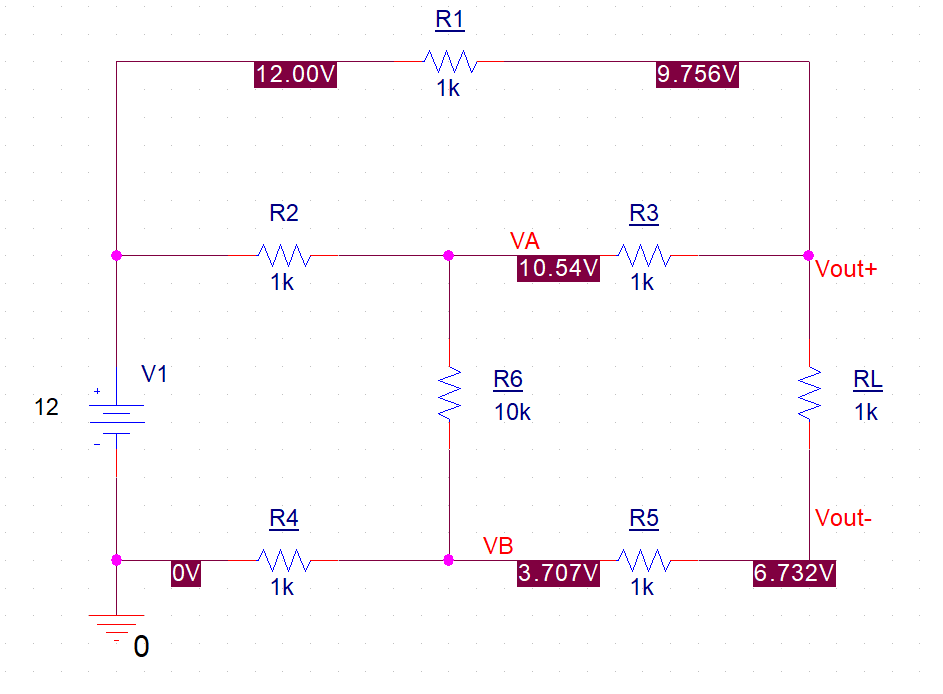
\includegraphics[height=10cm]{schematic}
	\caption{PSPICE simulation with voltage markers.}
	\label{fig:simulation}
\end{figure}

In Figure \ref{fig:simulation} the circuit shows the results of the PSPICE simulation and all of the nodal voltages. The nodal voltage at $V_A$ and $V_B$ were $10.54\,\si\volt$ and $3.707\,\si\volt$ respectively. The voltage at nodes $V_{out+}$ and $V_{out-}$ were measured at $9.756\,\si\volt$ and $6.732\,\si\volt$ respectively giving $V_{out}$ a voltage of $3.024\,\si\volt$. These perfectly aligned with the hand calculations done in the previous section.

%\subsubsection{PSPICE: DC Monte Carlo Simulation }
%
%In this section, include: 
%\begin{itemize}
%	\item A figure illustrating the Monte Carlo histogram extraction of the differential voltage ($V_{out}$) and the PDF.
%	\item  Briefly comment about the results and whether they agree with your hand calculations in the context of variations to the resistors.
%\end{itemize}


\section{Hardware Experiment: Results and Discussion}
%This section of the report should present what was done in hardware.  A reader should be able to recreate an experiment from the detail present.  One section discusses the equipment used in the experiment. The remaining sections discuss the results for each circuit.

The hardware portion of this exercise consisted of reading the resistances of each of the seven resistors and building the circuit. A measurement on each of the unknown nodes was taken using a multimeter.

\subsection{Equipment Used in the Laboratory}
%Write a short paragraph to detail the equipment used in the laboratory, and specific model numbers. Ideally, you should create a table of the equipment which should be referred to in text (See Table \ref{Table:Equipment} as an example).  The room location where the experiment was performed should be included.  Note that this should be a part of all Tech Memos, as it is an essential piece for other users to replicate your experiment.  \textbf{As you will be likely using the same equipment throughout the term, once the text/tables are established, you may reuse the information with the permission of your instructor/TA. Again, cite your first lab report as a reference.}

\begin{table}[htbp]
	\setlength{\tabcolsep}{14pt}
	\caption{Equipment/Software required for Lab 1.}
	\label{Table:Equipment}
	\begin{center}
	%\begin{tabular}{llllll}
		\begin{tabular}{|c||c|c|c|c|}
			\hline
			Item & Tool & Room      \\
			\hline
			Simulation & OrCAD Capture CIS & 09-3200   \\
			\hline  
			DC Power Supply & Agilent E3631A   & 09-3200 \\ 
			\hline 
			Multimeter & Agilent 34401A & 09-3200 \\
			\hline
			%				Oscilloscope & Textronix TDS2012C & 09-3200  \\
			%				\hline
			%				Oscilloscope & Agilent DSO 33120A & 09-3170  \\
			%				\hline
			%				
		\end{tabular}
	\end{center}
\end{table}

PSPICE Capture CIS was used to create the circuit and the perform the simulation. The DC Power Supply shown in Table \ref{Table:Equipment} was used in the hardware portion to power the circuit. The multimeter shown was used to measure the voltage and resistances across each of the resistors.

\subsection{Hardware Results/Discussion}	
%Begin the section by including the experimental values of the resistors as illustrated in Table \ref{Table:Lab2Resistors}. Introduce the table in the text and briefly discuss the variation in resistance. Note that the nominal values are the ones provided in the lab handout and used in PSPICE.   

The resistances of all seven resistors were measured and recorded using the resistance tool on the multimeter.

\begin{table}[h!]
  	\caption{Resistor Table}
	\begin{center}
  		\label{Table:Lab2Resistors}
  		
  		\begin{tabular}{|c||L|L|c|}
  			\hline
  			Resistor & Nominal Value (\si{\kilo\ohm})& Measured Value (\si{\kilo\ohm}) & Tolerance (\si{\percent})   \\
  			\hline
  			$R_1$ & 1 & 0.983 & 5  \\	 \hline 
  			$R_2$ & 1 & 0.983 & 5 \\	 \hline 
  			$R_3$ & 1 & 0.987 & 5 \\	 \hline 
  			$R_4$ & 1 & 0.981 & 5 \\	 \hline 
  			$R_5$ & 1 & 0.982 & 5 \\	 \hline 
  			$R_6$ & 10 & 9.95 & 5 \\	 \hline
  			$R_L$ & 1 &  0.986 & 5 \\	 \hline 
  		\end{tabular}
  	\end{center}
\end{table}

The small variance from nominal and measured values are due to phyiscal variations in the resistors. They are all within specified tolerances.
  	
\subsection{Hardware Results Summary}
%The lab handout calls for the measuring equivalent resistance between two points in the circuits to verify the wiring.  Report the values that were obtained experimentally.  Next, include the following table per the lab documentation. Briefly summarize it. Include a discussion of the \textbf{percent error} between theory and experiment.

The voltages relative to ground were measured for each of the unknown nodes, $V_A$, $V_B$, $V_{out+}$, and $V_{out-}$. The equivalent resistance accross the power supply was measured to be $3.231\,k\si\ohm$. The equivalent resistance accross $R_L$ was measured at $0.915\,k\si\ohm$.
  
\begin{table}[h!]
	\caption{Summary of nodal voltages for Lab 2.}
	\label{Table:Lab2DCVoltages}
	%\begin{tabular}{llllll}
	\begin{center}
		\begin{tabular}{|c||L|c|c|L|}
			\hline
			Voltage & Hand Calculations (\si{\volt}) &  PSPICE (\si{\volt})& Hardware (\si{\volt}) & Percent Error With Hand Calc. (\si{\percent})   \\
			\hline
			$V_A$ & 10.54 & 10.54 & 10.54 & 0 \\	 \hline 
			$V_B$ & 3.707 & 3.707 & 3.697 & 0.27 \\	 \hline 
			$V_{out+}$ & 9.756 & 9.756 & 9.764 & 0.08 \\	 \hline
			$V_{out-}$ & 6.732 & 6.732 & 6.723 & 0.13 \\	 \hline 
			$\Delta V_{out}=V_{out+}-V_{out-}$ & 3.024 & 3.024 & 3.040 & 0.53 \\	 \hline
		\end{tabular}
	\end{center}
\end{table}

Table \ref{Table:Lab2DCVoltages} shows a very slight error in the measured voltages of the unknown nodes. This is due to the fact that the equipment used provided very little room for error.

\section{Conclusion}
%Provide a 1 paragraph summary of the laboratory experiment.  What were the major conclusions for each part of the experiment?  Also did the theory agree with the experiment?  The conclusion is a revised version of the abstract.

This laboratory experiement made students more comfortable with PSPICE Capture CIS software and simulation by having students design and simulate a more complex circuit. The simulation in PSPICE was compared to hand calculations. Hand calculation were obtained through nodal analysis or mesh analysis. Finally the circuit was constructed on a bread board and the unknown nodes were measured using a multimeter. Results were compared to the calculation obtained in the prelab.

\section{Acknowledgments}
\begin{itemize}
	\item wikibooks.org helped with the \LaTeX\;code.
	\item tex.stackexchange.com helped with the circuit diagram in \LaTeX.
	\item Petre Tumbar and Walter Sigel were present in the lab for the prelab and experiment.
\end{itemize}


	
	\textbf{Your report should include references to appropriate pages in the text, as well as any other sources, websites/etc. consulted in the preparation of the report.}
\begin{thebibliography}{9}
	\bibitem{AlexanderSadiku}
	C.K. Alexander, and M.K.O. Sadiku,
	\emph{Fundamentals of Electric Circuits, 4th Edition},
	McGraw Hill, pp. xx-yy(EDIT), 2009.
	\bibitem{OldLab}
A. Student,
	\emph{EEEE 281 Lab 1 Tech Memo},
	page xx-yy, submitted Month, Day, 2015.
	\bibitem{RommelLab}
	S. Rommel,
	\emph{EEEE 281 Lab 1 Lecture notes},
	slides xx-yy, Spring 2015.
\end{thebibliography}

\end{document}



